\documentclass [pdftex,12pt] {report}
\usepackage [utf8]{inputenc}
\usepackage [french] {babel}
\usepackage[pdftex]{graphicx}
\usepackage{sidecap}
\usepackage{float}
\usepackage{natbib,hyperref}
\usepackage{indentfirst}
\usepackage[T1]{fontenc} 
\usepackage{amsfonts}
\usepackage{listings}
\usepackage{color}
\usepackage{textcomp}
\definecolor{gray}{rgb}{0.4,0.4,0.4}
\definecolor{darkblue}{rgb}{0.0,0.0,0.6}
\definecolor{cyan}{rgb}{0.0,0.6,0.6}

\lstset{
  basicstyle=\ttfamily,
  columns=fullflexible,
  showstringspaces=false,
  commentstyle=\color{gray}\upshape
}

\lstdefinelanguage{XML}
{
  morestring=[b]",
  morestring=[s]{>}{<},
  morecomment=[s]{<?}{?>},
  stringstyle=\color{black},
  identifierstyle=\color{darkblue},
  keywordstyle=\color{cyan},
  morekeywords={xmlns,version,type}
}

\def\wl{\par \vspace{\baselineskip}}
\renewcommand{\lstlistingname}{Code}
\newcommand{\HRule}{\rule{\linewidth}{0.5mm}}

\bibliographystyle{unsrt}
\begin {document}

% Include the front page
\begin{titlepage}
\begin{center}

% Upper part of the page. The '~' is needed because \\
% only works if a paragraph has started.

\includegraphics[width=0.15\textwidth]{./resources/logo}~\\[1cm]

\textsc{\LARGE Université de Bordeaux 1}\\[1.5cm]

\textsc{\Large {Projet de Programmation}}\\[0.5cm]

% Title
\HRule \\[0.4cm]
{ \huge \bfseries Application CampusUB1}\\[0.4cm]

\HRule \\[1.5cm]

% Authors, clients and supervisor
\begin{minipage}{0.4\textwidth}
\begin{flushleft} \large
\emph{Auteurs:} \\
Elyas \textsc{Ben Hadj Yahia}\\
Ryan \textsc{Herbert}\\
Paul \textsc{Maribon-Ferret}\\
Stefan \textsc{Mijatovic}\\
Tatiana \textsc{Rocher}
\end{flushleft}
\end{minipage}
\begin{minipage}{0.4\textwidth}
\begin{flushright} \large
\emph{Clients:} \\
Fabien \textsc{Baldacci}\\
Arnaud \textsc{Casteigts}\\
\emph{\\Encadreur:} \\
Xavier \textsc{Blanc}
\end{flushright}
\end{minipage}

\vfill

% Bottom of the page
{\large \today}

\end{center}
\end{titlepage}

\newpage

\begin{abstract}
Ce document décrit le travail réalisé dans le contexte de notre projet de programmation. Le but de ce projet est de réaliser une application Android permettant d'accéder aux informations pertinentes des différents établissements du campus (Laboratoires, Universités, Ecoles). L'utilisateur choisit les établissements pour lesquels il veut accéder aux informations (dans un premier temps il n'y aura que Bordeaux 1 et LaBRI). L'application permet ensuite d'accéder aux annonces d'événements (en offrant la possibilité des les ajouter à l'agenda) et aux annuaires (en offrant la possibilité d'ajouter aux contacts du téléphone) sélectionnés. \\
L'idée est donc de rendre les informations liées aux établissements choisis plus faciles d'accès via un smartphone Android, afin de répondre à un besoin en déplacement, en donnant la possibilité d'enregistrer les informations importantes, et de les intégrer aux applications natives du téléphone, pour permettre une utilité de l'application lorsqu'une connexion internet n'est pas disponible.
\end{abstract}


\vspace{2cm}
\tableofcontents
\newpage 

\chapter{Etude de l'existant}
\section{Références}


\subsection{Android Application Development}
L'ouvrage \emph{Android Application Development}~\cite{AndroidBook} est considéré comme l'une des références majeures dans le domaine du développement des applications sur Android.
Il présente notamment l'architecture du système d'opération Android, ainsi que les différentes phases de développement des applications utilisateurs.

\subsection{Site officiel de la SDK Android}
Le site officiel de la SDK Android~\cite{AndroidSDK} met à disposition des développeurs une panoplie d'outils et de références.
Ce site présente ses divers services, notamment les API d'Android et autres services de Google. On y trouve aussi plusieurs domaines d'application utilisés aujourd'hui qu'on peut intégrer dans notre application.

\subsection{Article sur les applications mobiles des universités}
Cet article sur les applications mobiles des universités~\cite{Article} décrit les différentes contraintes liées au développement des applications mobiles d'universités. Etant donné que les étudiants sont de plus en plus équipés de smartphones, il devient intéressant de mettre en place une application mobile qui offre divers services utiles et faciles d'accès.


\section{Applications existantes}

\subsection{uMontréal}
Cette application propriétaire de l'université de Montréal~\cite{uMontreal} met à disposition de ses étudiants de nombreux services, tels que des flux d'actualités, un annuaire, un calendrier, et le plan du campus.

\subsection{Plateforme Blackboard}
Cette plateforme de développement est utilisée par la majorité des applications campus mobiles aux Etats-Unis~\cite{Blackboard}. On considère par exemple iStandford~\cite{iStanford}, application Android qui présente de nombreux services (internes et externes), dans la même philosophie que l'application uMontréal.

\subsection{gReader, lecteur de flux RSS}
Ce lecteur de flux RSS~\cite{gReader} offre une interface sobre et pratique pour gérer les abonnements aux flux RSS. Notre développement de l'interface graphique pourra s'inspirer du système des onglets et des toolbars de cette application.

\subsection{Lecteurs de flux RSS open-source}
Il existe déjà plusieurs lecteurs de flux RSS open-source, tels que Feedgoal~\cite{Feedgoal} et Android-RSS~\cite{Android-RSS}. les deux étant sous license GNU GPL (v2 et v3, respectivement). On pourra étudier s'il est rentable de reprendre quelques modules, ou de repartir sur notre propre base.


\section{Ressources existantes}

\subsection{LDAP}
Le protocole LDAP est une ressource potentiellement importante à la conception de notre application, notamment pour la mise en oeuvre de l'annuaire. LDAP signifie Lightweight Directory Access Protocol; c'est donc un protocole conçu uniquement pour les annuaires, et l'annuaire du LaBRI s'avère être conforme aux normes LDAP.
Ce sera donc une des technologies importantes à explorer afin de réaliser une réponse robuste au parsage de l'annuaire du LaBRI.\\
Nous nous sommes posés la question de l'accessibilité de l'annuaire venant de l'extérieur, au format LDAP, cependant nous avons trouvé une page d'aide sur un forum du LaBRI\cite{labriForum} qui pourrait donner une solution éventuelle.

\subsection{HTTP/HTML}
Une alternative au protocole LDAP serait d'effectuer des requêtes HTTP, afin de parser des pages HTML. Cette méthode pourrait répondre aux besoins de parser les annuaires dont il en est question, si jamais nous ne pouvons nous reposer sur le LDAP. Le problème posé par cette méthode repose dans la robustesse de la solution. C'est-à-dire qu'un changement de l'implémentation des pages (changement/mise à jour des balises, ou même un changement de forme) pourrait rendre l'application inutilisable. L'utilisation de cette méthode demande énormément de travail de généricité du parsage des pages.
Ceci pose plusieurs problèmes, notamment sur l'imprévisibilité des changements potentielles dans les pages. Il est impossible de prévoir à 100\% les modifications qui pourraient avoir lieu sur les pages, et donc l'application pourrait rapidement devenir inutilisable. Il sera nécessaire de s'inspirer voire de réutiliser certains codes de web crawlers open source afin d'assurer d'avoir une application aussi robuste qu'elle puisse l'être en parsant des pages HTML.


\subsection{Analyse textuelle}
Au cours de l'implémentation de cette application, nous pourrions être amenés à effectuer de l'analyse textuelle sur des textes afin d'en extraire les informations dont nous avons besoin, par exemple si une date n'est pas au sein d'une balise facilement repérable/exploitable. Il faudra donc peut-être tenter d'extraire des dates des textes disponibles. Celà pose plusieurs problèmes:
\begin{itemize}
\renewcommand{\labelitemi}{$\bullet$}
  \item Le texte peut faire référence à un événement passé, simplement à titre informatif, auquel cas, une date extraite n'aurait pas nécessairement de valeur à l'exploitation avec notre application.
  \item Le texte peut contenir plusieurs dates, faisant référence à plusieurs événements passés, présents, ou futurs et il sera donc difficile d'exploiter les informations et de découper le texte en plusieurs événements, ou encore d'extraire la date pertinente à l'événement.
  \item Le texte peut ne contenir aucune date, n'étant simplement qu'une information quelconque.
\end{itemize}
\wl Les événements inscrits dans les flux RSS du site de Bordeaux 1 possèdent une balise \emph{pubDate}, qui devrait faire référence à la date de publication des articles, mais nous avons remarqué que pour la plupart des articles (notamment pour toutes les soutenances), cette date a été modifiée pour correspondre à la date de la soutenance. Cependant, ce n'est pas toujours le cas pour l'horaire. Certains articles possèdent des horaires qui correspondent à celle de l'événement (comme pour les soutenances, par exemple), mais d'autres ont un horaire qui ne correspond pas avec l'horaire de l'événement. Nous avons donc tiré la conclusion que l'horaire correspond parfois à l'horaire de publication de l'article. \\
Il sera donc possible de comparer les dates et horaires extraites par analyse textuelle avec les informations contenues dans la balise \emph{pubDate} afin d'augmenter le taux de réussite de la proposition de date au moment de l'ajout dans l'agenda du smartphone. \\

\lstset{language=XML}
\begin{lstlisting}[frame=single, caption=Extrait d'un flux RSS de Bordeaux1 (29/01/2013), label=xml1]
<item>
  <title>Trophees du sport</title>
  <link>...</link>
  <description>
	Pour la 3e annee consecutive...
  </description>
  <content:encoded>
    <![CDATA[
      Ils seront recompenses a l occasion des Trophees du sport
      le jeudi 31 janvier 2013 a 18h dans l Atrium...
    ]]>
  </content:encoded>	
  <pubDate>Thu, 31 Jan 2013 15:08:00 +0100</pubDate>
</item>
\end{lstlisting}

\wl Sur cet exemple, l'heure qui apparait dans la balise \emph{pubDate} ne correspond pas à celle de l'événement; il va donc falloir analyser la description pour essayer de trouver l'horaire correspondant (ici 18h). \\

Il existe plusieurs outils utiles à l'implémentation d'une solution à ce problème, notamment JFlex/CUP qui, d'après un livre d'Android~\cite{ProgAndroid} reste une solution possible. Ces outils ressortent pour nous, car leur utilisation nous est déjà familière. Ces outils cumulés avec les informations extraites d'un livre d'analyse textuelle~\cite{analyseTextuelle}.\\
Etant donné ces problèmes, nous devrons surement trouver une approximation au problème, car nous ne pourrons proposer la bonne date à chaque fois qu'un utilisateur souhaite ajouter un élément à son agenda. Il sera donc parfois nécessaire de créer un menu qui s'ouvre automatiquement afin de proposer les dates qui ont été détectées par notre algorithme, et qui donne la possibilité à l'utilisateur de saisir sa propre date (ainsi on réduit de manière conséquente la marge d'erreur sur l'entrée finalisée dans l'agenda). \\



\chapter{L'Application CampusUB1}
\section{Aperçu de l'application}

\subsection{Actualités}
Une des fonctionalités principales de l'application est la récupération, l'affichage et l'enregistrement des événements dans le calendrier de l'utilisateur. 
Pour cela, nous prévoyons de récuperer les flux RSS les plus utiles de l'université Bordeaux 1\cite{fluxBDX1}, notamment les flux disponibles sur la page d'accueil du site de l'université (dont les actualités).
En ce qui concerne le site du LaBRI, il n'y a aucun flux RSS et il faudra donc parser directement du HTML.

\subsection{Annuaire}
Il sera également possible de consulter les annuaires des établissements concernés, afin d'en extraire les informations désirées et les ajouter aux contacts du smartphone.
Afin d'implémenter l'annuaire au sein de notre application Android, il est évident qu'il faut exploiter les annuaires de Bordeaux 1~\cite{AnnuaireBdx1} et du LaBRI. En ce qui concerne le LaBRI, le serveur LDAP n'est pas accessible depuis l'extérieur (sans authentification).Nous devrons donc intégrer l'annuaire à travers des requêtes GET, dans le but de parser les résultats obtenus. Pour le moment ceci semble être la meilleure solution envisageable. L'accès sans authentification au serveur LDAP de l'université de Bordeaux1 nous est permis, ce qui facilitera grandement l'intégration de la recherche dans l'annuaire pour cet établissement, ainsi que la maintenabilité du logiciel.


\subsection{Utilitaires}
\subsubsection{Plan du campus}
Dans un deuxième temps, nous prévoyons de mettre en place un plan du campus, potentiellement intégré à l'application Maps du smartphone.
Ce service permettrait donc à l'utilisateur d'avoir un aperçu plus détaillé du campus en affichant les différents bâtiments et leur noms.
On poura éventuellement aussi afficher les emplacements des différents services dédiés aux étudiants (cafétéria, restaurant universitaire, bibliothèque universitaire, ...).

\subsubsection{Emploi du temps}
Un autre service qui pourrait être très utile en particulier pour les étudiants de Bordeaux1 est l'accès et la sauvegarde locale de leur emplois du temps en fonction de leurs filières, des groupes, et des différentes options suivies. 
Pour cela, nous parserons les fichiers XML des emplois du temps utilisant la plateforme Celcat\cite{EdTxml}, afin de mettre à disposition une copie locale de l'emploi du temps dans l'agenda du smartphone.

\chapter{Analyse des besoins}

Nous allons analyser dans ce chapitre les différents besoins fonctionnels et non-fonctionnels de notre application.\\
Nous allons donc utiliser un système de points pour évaluer la difficulté des tâches. On se basera sur une séquence de Fibonacci arrondie (1, 2, 3, 5, 8, 13, 20, 40, 60, 100), avec 100 reflétant une tâche d'une grande difficulté.\\
Les priorités des besoins sont classées sur cette échelle: optionnel, faible, moyen, important, vital.
\section{Besoins fonctionnels}
\subsection{Fonctionnalités principales}
\subsubsection{Choix de l'établissement}
Etant donné que l'application présentera des services en commun à plusieurs établiseements, l'utilisateur doit pouvoir s'abonner aux établissements de son choix, s'il souhaite accéder à leurs propres informations [Fig.~\ref{fig:01}]. \\

\begin{itemize}
\renewcommand{\labelitemi}{$\bullet$}
\item Priorité: vital
\item Difficulté: 1/100
\item Risques: mise à jour des liens si les adresses des établissements sont modifiées.
\item Validation: s'assurer que les sélections et les changements d'établissements s'effectuent correctement.
\end{itemize}

\subsubsection{Gestion des actualités}
En accédant au menu des actualités, l'utilisateur disposera d'une interface à travers laquelle il recevra le flux des actualités des établissements auxquels il est abonné. Par défaut il aura alors la possibilité de voir les événements propres aux établissements auxquels il s'est abonné. Il pourra à tout moment changer de catégorie grâce au menu des catégories [Fig.~\ref{fig:04}] depuis la même fenêtre. De plus, il peut choisir entre voir la totalité des actualités des établissements auquels il a souscrit, ou voir uniquement les actualités propres aux établissements qu'il a sélectionné dans les filtres.  [Fig.~\ref{fig:03}]. L'utilisateur doit pouvoir lire l'annonce de ces événements [Fig.~\ref{fig:04}], et doit pouvoir facilement rajouter cet événement au calendrier de son smartphone (Google Calendar). Cette action redirigera l'utilisateur vers le calendrier, dans lequel l'événement sera créé avec les informations récoltées. L'utilisateur pourra donc modifier, valider ou annuler la procédure. \\

\begin{itemize}
\renewcommand{\labelitemi}{$\bullet$}
\item Priorité: vital
\item Difficulté: 40/100
\item Difficultés techniques: extraction des informations pertinentes.
\item Risques: changement de structure du contenu à parser (flux RSS et pages HTML).
\item Validation: assurer l'intégrité des informations extraites.
\end{itemize}

\subsubsection{Accès à l'annuaire}
L'utilisateur doit pouvoir effectuer facilement les tâches suivantes:\\
\begin{itemize}
\renewcommand{\labelitemi}{$\bullet$}
\item Rechercher un contact dans l'annuaire par son nom et/ou prénom.
\item Visualiser les informations d'un contact.
\item Rajouter un contact à la liste des contacts de l'utilisateur (créer un nouveau contact ou éditer existant).
\item Envoyer un mail au contact.
\item Appeler la personne (si un numéro de téléphone est disponible).
\end{itemize}

\wl La recherche de personnes dans l'annuaire se fera en fonction des établissements auquels l'utilisateur s'est abonné. On pourra donc choisir grâce à un filtre entre rechercher une personne dans l'annuaire propre à un ou plusieurs établissements, ou la rechercher dans tous les annuaires.
Lors de l'ajout d'un contact, l'utilisateur sera redirigé vers la page de création d'un nouveau contact, dans laquelle les champs pertinents seront pré-remplis, en fonction des informations collectées. L'utilisateur pourra donc modifier, valider ou annuler la procédure. \\

\begin{itemize}
\renewcommand{\labelitemi}{$\bullet$}
\item Priorité: vital
\item Difficulté: 40/100
\item Difficultés techniques:
\begin{itemize}
\item Avec LDAP: mise en place du protocole.
\item Sans LDAP: parsage des informations.
\end{itemize} 
\item Risques: changement de structure du contenu à parser.
\item Validation: assurer l'intégrité des informations extraites.
\end{itemize}

\subsubsection{Mises à jour}
Notre application pouvant fonctionner hors connexion, les mises à jour de flux RSS étant de type pull, il est important de proposer les mises à jour sur les flux que nous parsons. Par exemple après une longue période sans connexion nous pourrons sauter sur l'occasion de proposer des mises à jour des flux dès que l'utilisateur ouvre l'application et qu'une connexion internet est disponible. Une autre solution serait de mettre à disposition un bouton \emph{refresh} pour que l'utilisateur puisse effectuer une demande de mise à jour (option préférable pour les personnes ayant un forfait internet limité, ou encore pour l'utilisation à l'étranger). Nous pourrions également proposer une solution intermédiaire, où l'application effectue des mises à jour régulières lorsqu'elle est connectée sur un réseau via le WiFi, mais requiert une demande explicite si le réseau est de type 3G. \\
L'application devra garder en mémoire les derniers éléments téléchargés pendant un mois après la date de l'événement (durée à revoir éventuellement). Ainsi lorsque l'on n'a pas accès à internet, on pourra accèder à ceux-ci. De plus, lors des mises à jour, on téléchargera uniquement les nouveaux événements. Ceci permettra à l'application d'économiser du temps d'éxécution, et potentiellement du crédit à l'utilisateur. \\

\begin{itemize}
\renewcommand{\labelitemi}{$\bullet$}
\item Priorité: important
\item Difficulté: 40/100
\item Risques: mauvaise gestion de la mémoire.
\item Difficultés techniques: éviter de télécharger de nouveau des informations déja collectées.
\item Validation: vérifier l'intégration des nouvelles informations.
\end{itemize}


\subsection{Fonctionnalités secondaires}
Dans un deuxième temps, nous comptons implémenter quelques optionalités supplémentaires, qui ne rentrent pas dans le cadre du projet initial, mais qu'on estime être assez pratiques et utiles, et permettront de compléter l'application.

\subsubsection{Abonnements et filtrage d'informations}
Après avoir choisi lors du premier démarrage de l'application, les établissements auprès desquels l'utilisateur souhaite s'abonner,
il pourra à tout moment revenir sur son choix à travers le menu des préférences. Il pourra également en fonction de ses abonnements actifs visualiser la totalité des informations propres à un, plusieurs ou tous les établissements grâce à un outil de filtrage. Cet outil se présente sous la forme d'une fenêtre quasiment identique à celle du choix des abonnements ~[Fig.~\ref{fig:03}] et sera accessible uniquement depuis l'écran d'acceuil. \\

\begin{itemize}
\renewcommand{\labelitemi}{$\bullet$}
\item Priorité: optionnel
\item Difficulté: 60/100
\item Difficultés techniques: s'assurer que l'abonnement simultané à un grand nombre d'établissements n'ait aucun impact sur la stabilité de l'application.\\
\item Risques: saturation trop rapide de la mémoire cache.
\item Validation: affichage cohérent des informations liés aux abonnements actifs.
\end{itemize}

\subsubsection{Emploi du temps}
L'utilisateur étudiant doit pouvoir récupérer son emploi de temps du semestre et l'intégrer à Google Calendar. Il doit pouvoir indiquer sa filière, et éventuellement ses cours et ses groupes. \\

\begin{itemize}
\renewcommand{\labelitemi}{$\bullet$}
\item Priorité: optionnel
\item Difficulté: 60/100
\item Difficultés techniques: extraction des informations en fonction du choix de l'utilisateur.
\item Risques: changement du format de l'emploi du temps.
\item Validation: assurer l'intégrité des données extraites.
\end{itemize}

\subsubsection{Plan du campus}
L'utilisateur pourra naviguer sur le plan du campus en utilisant Google Maps. L'utilisateur disposera des pointeurs vers les bâtiments principaux du campus. \\

\begin{itemize}
\renewcommand{\labelitemi}{$\bullet$}
\item Priorité: optionnel
\item Difficulté: 60/100
\item Difficultés techniques: maîtriser l'API de Google Maps.
\end{itemize}



\section{Besoins non fonctionnels}
\subsection{Besoins de performance}
L'application CampusUB1 est destinée à toute personne étudiant ou travaillant sur le campus de l'université. Elle devra donc être capable de tourner sur les derniers smartphones, tout en restant compatible avec des smartphones plus anciens et donc moins puissants puisque tout étudiant n'a pas forcément les moyens d'aborder un smartphone récent ayant une forte puissance de calcul et une grande quantité de RAM. CampusUB1 ne sera donc pas gourmande en ressources et pourra exécuter ces services de manière assez rapide même sur les smartphones moins performants.\\
Nous testerons l'application sur les appareils suivants: LG Optimus 2X (P990), Sony Xperia S, Samsung Galaxy S3.\\

\begin{itemize}
\renewcommand{\labelitemi}{$\bullet$}
\item Priorité: faible
\item Difficulté: 40/100
\item Difficultés techniques: bonne gestion de l'espace mémoire et de l'actualisation.
\item Risques: implémention complexe et potentiellement longue.
\item Validation: vérification que l'utilisation reste assez fluide et ne consomme pas beaucoup de ressources (à préciser un seuil de consommation de RAM).
\end{itemize}  

\subsection{Besoins de fiabilité}
Etant donné que les différents services mis à disposition par CampusUB1 à ses clients s'avèrent souvent être d'un besoin professionnel, il est essentiel que les données affichées soient cohérentes et en accord avec les données d'origine. Si un chercheur du LaBRI recherche depuis notre application le numéro de la salle où a lieu sa conférence, il a tout intérêt à récupérer une information correcte. CampusUB1 ne peut tout de même pas garantir l'exactitude de toutes les informations données et ne se tient donc pas responsable d'éventuelles erreurs, sachant que l'application se base sur des algorithmes de reconnaissance de textes qui peuvent eux-mêmes être erronés d'origine. Il est évident que certaines questions de sécurité courantes se posent sachant que l'application nécessite une connection à internet continue, mais vu que CampusUB1 utilise uniquement des données publiques dans les services qu'elle fournit, la question de confidentialité des données ne se pose pas. \\

\begin{itemize}
\renewcommand{\labelitemi}{$\bullet$}
\item Priorité: moyen
\item Difficulté: 60/100
\item Difficultés techniques: fiabilité de l'algorithme d'analyse textuelle pour détecter les dates des événements.
\item Risques: création d'un événement avec des données erronées.
\item Validation: simulation de l'algorithme d'analyse textuelle sur suffisamment de données pour avoir un taux de réussite acceptable (à déterminer).
\end{itemize}  

\subsection{Besoins d'intégrité de données}
CampusUB1 doit accéder à certaines ressources personnelles du client pour pouvoir fonctionner, ce qui pose un problème de protection des données. Le calendrier et le répertoire du client sont les ressources auxquelles l'application est susceptible d'accéder, et on devra s'assurer que toute perte éventuelle de données déjà existantes ne soit pas engendrée par une erreur provenant de l'application. L'erreur humaine étant évidemment toujours possible. Toute modification éventuelle de données privées de l'utilisateur se fera donc impérativement avec son avis. \\

\begin{itemize}
\renewcommand{\labelitemi}{$\bullet$}
\item Priorité: moyen
\item Difficulté: 40/100
\item Risques: perte des informations existantes sur le smartphone.
\item Validation: monitoring du comportement de l'application.
\end{itemize} 


\subsection{Besoins organisationnels}
Etant donné que nous travaillerons sur la plateforme Android, le langage Java nous est imposé vu que l'API Android est fournie en Java.
L'IDE dans lequel nous avons choisi d'implémenter notre application est Eclipse pour de nombreuses questions pratiques. Les développeurs d'Android disposent d'un plugin officiel pour Eclipse, qui facilite le travail du développeur en lui fournissant une panoplie d'outils tels que les différentes perspectives dont celle de débogage qui nous sera très utile. Ce plugin comporte également un émulateur d'appareils Android, ce qui nous permettra de facilement tester l'application sur une multitude d'appareils virtuels. De plus, l'API Android est très documentée et est maintenue fréquemment.



\chapter{Diagrammes de fonctionnement}

\section{Fonctionnalités de l'application}

\begin{figure}[h]
  \center
  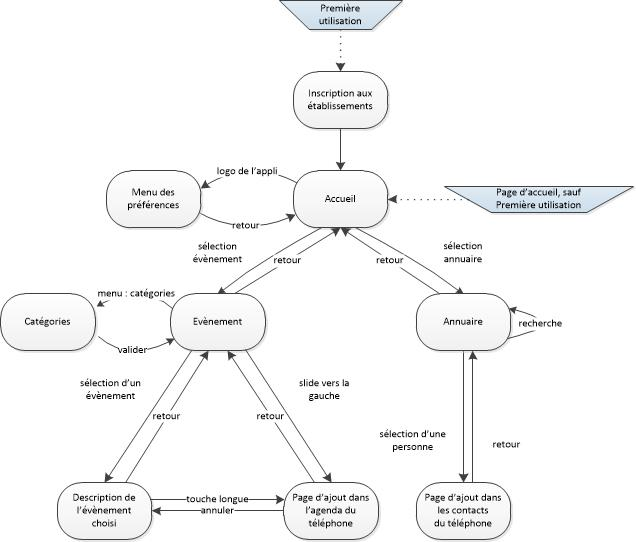
\includegraphics[width=0.92\textwidth]{resources/features1.jpg}
\end{figure}

\newpage

Le diagramme ci-dessus présente toutes les actions réalisables par l'utilisateur et leurs enchaînements.
Lorsque l'utilisateur démarre l'application pour la première fois, il choisit l'établissement auprès duquel il veut s'abonner.
Ce choix est alors retenu, et cette étape est donc omise lors des futurs démarrages de l'application. Une option existera tout de même pour modifier les abonnements si nécessaire. Depuis l'écran d'accueil, l'utilisateur pourra alors accéder aux services de son choix et pourra à tout moment revenir en arrière facilement. \\

\begin{figure}[h]
	\center
	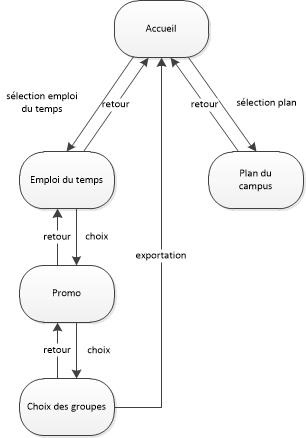
\includegraphics[width=0.6\textwidth]{resources/features2.jpg}
\end{figure}

Le diagramme ci-dessus présente les services offerts pour l'établissement Bordeaux1. Ces services seront accessibles quand l'utilisateur sera abonné à Bordeaux1.

\section{Diagramme des mises à jour}

\begin{figure}[h]
  \center
  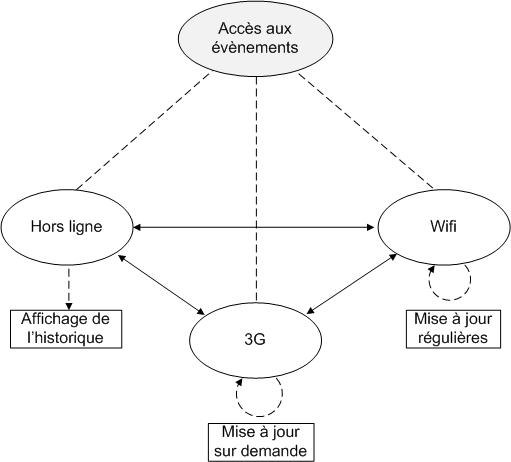
\includegraphics[width=0.6\textwidth]{resources/state_diagram.jpg}
\end{figure}

Le diagramme de mises à jour représente les différents modes de connection dans lesquels on peut se trouver lorsqu'on accède aux événements. Il y a trois modes possibles gérés par le téléphone :\\
\begin{itemize}
\renewcommand{\labelitemi}{$\bullet$}
 \item Hors Ligne : pas d'accès à internet.
 \item 3G :  accès au réseau de données mobiles (lent).
 \item WiFi : accès à un réseau sans-fil (rapide).
\end{itemize}

\newpage

\section{Diagramme de Gantt}
Le diagramme de Gantt suivant présente une première estimation de la répartition des tâches sur le déroulement du projet.

\begin{figure}[h]
  \center
  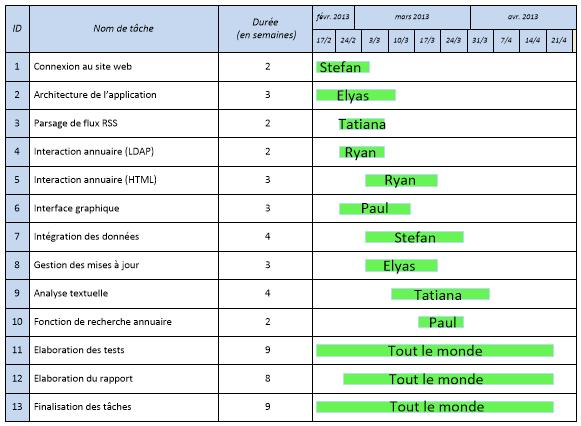
\includegraphics[width=1.0\textwidth]{resources/gantt.jpg}
\end{figure}

Chaque ligne représente une tâche à effectuer, une estimation de sa durée, et son attribution. \\


\chapter{Tests et Validation}
  
  \section{Test 01: Choix de l'établissement}
    \begin{enumerate}
    \item Démarrer l'application pour la première fois, un menu vous sera proposé pour effectuer le choix de l'établissement~[Fig.~\ref{fig:01}].
    \item Sélectionnez les établissements auxquels vous voulez vous abonner.
    \end{enumerate}

    \underline{Résultat attendu}: Vous serez redirigé vers le menu principal de l'application.

  \section{Test 02: Maintien du choix de l'établissement}
    \begin{enumerate}
    \item Quittez l'application, et redémarrez-la.
    \end{enumerate}

    \underline{Résultat attendu}: L'application aura sauvegardé vos choix d'établissement, et vous redirigera à la page d'accueil de l'application.

  \section{Test 03: Evénements}
    \begin{enumerate}
    \item Une fois les abonnements configurés, sélectionner le menu des événements dans le menu principal~[Fig.~\ref{fig:02}].
    \end{enumerate}

    \underline{Résultats attendus}:
    \begin{itemize}
    \item Si l'application est connectée à Internet: Les événements de tous les établissements auxquels l'application est abonnée sont affichés~[Fig.~\ref{fig:04}].
    \item Sinon: Les événements ayant déjà été téléchargés sont affichés.
    \end{itemize}

  \section{Test 04: Validité des informations extraites d'un évenement}
    \begin{enumerate}
    \item Depuis l'accueil, appuyer sur Evénements.
    \item Naviguer dans la liste des événements.
    \item Appuyer sur un événement afin d'afficher la vue détaillée~[Fig.~\ref{fig:06}].
    \item Effectuer une touche longue sur l'écran.
    \end{enumerate}

    \underline{Résultat attendu}: Les propositions d'informations correspondent aux informations contenues dans l'évenement.

  \section{Test 05: Ajout d'un événement au smartphone}
    \begin{enumerate}
    \item Effectuer le Test 04
    \item Valider l'ajout de l'événement.
    \end{enumerate}

    \underline{Résultat attendu}: L'événement sera ajouté à l'agenda du téléphone.


  \section{Test 06: Annuaire}
    \begin{enumerate}
    \item Sélectionner Annuaire dans le menu d'accueil.
    \end{enumerate}

    \underline{Résultats attendus}:
    \begin{itemize}
    \item Si l'application est connectée à Internet: on arrive sur l'écran de la~[figure~\ref{fig:07}].
    \item Sinon : un toast nous prévient qu'on est déconnecté.
    \end{itemize}

  \section{Test 07: Rechercher dans l'Annuaire}
    \begin{enumerate}
    \item Accéder à l'annuaire à partir du menu principal.
    \item Ecrire dans la barre de recherche~[Fig.~\ref{fig:08}], cela affichera tous les contacts qui correspondent à la recherche, parmis les établissement auxquels l'application est abonnée.
    \end{enumerate}

    \underline{Résultat attendu}: Le nombre de résultats se réduit à ceux qui correspondent à ce qui est écrit dans la barre de recherche.

  \section{Test 08: Validité des informations extraites}
    \begin{enumerate}
    \item Depuis l'accueil appuyer sur Annuaire
    \item Naviguer dans l'annuaire.
    \item Appuyer sur un contact afin d'afficher la vue détaillée.
    \item Effectuer une touche longue sur l'écran.
    \item Sélectionner \emph{Ajouter contact}.
    \item Sélectionner \emph{Ajouter un nouveau contact} ou \emph{Editer un contact existant}.
    \end{enumerate}

    \underline{Résultat attendu}: Les informations extraites correspondent aux informations contenues dans le contact.

  \section{test 09: Ajout d'un contact au téléphone}
    \begin{enumerate}
    \item Effectuer le Test 08.
    \item Valider l'ajout/l'édition du contact
    \end{enumerate}

    \underline{Résultat attendu}: Le informations se situe dans les contacts du téléphone.

  \section{Test 10: Appeler un contact}
    \begin{enumerate}
    \item Depuis le menu d'accueil appuyer sur Annuaire.
    \item Sélectionner un contact possédant un numéro de téléphone.
    \item Effectuer une touche longue sur l'écran.
    \item Sélectionner \emph{Appeler}
    \end{enumerate}

    \underline{Résultat attendu}: L'application démarrera un appel vers ce contact.

  \section{Test 11: Envoyer un mail à un contact}
    \begin{enumerate}
    \item Depuis le menu d'accueil appuyer sur Annuaire.
    \item Sélectionner un contact possédant un numéro de téléphone.
    \item Effectuer une touche longue sur l'écran.
    \item Sélectionner \emph{Envoyer un email}
    \end{enumerate}

    \underline{Résultat attendu}: L'application ouvre le gestionnaire d'email du téléphone avec le destinataire rempli avec l'adresse email du contact.

  \section{Test 12: Exporter un emploi du temps}
    \begin{enumerate}
    \item S'abonner à un établissement permettant l'exportation d'emplois du temps (ex: Bordeaux1).
<<<<<<< Updated upstream
    \item Depuis le menu d'accueil, appuyer sur "Export emploi du temps".
    \item Sélectionner un niveau d'études~[Fig.~\ref{fig:09}].
    \item Sélectionner une filière et un groupe~[Fig.~\ref{fig:10}].
    \item appuyer sur "Exporter"
=======
    \item Depuis le menu d'accueil, appuyer sur \emph{Export emploi du temps}.
    \item Sélectionner un niveau d'études.
    \item Sélectionner une filière et un groupe.
    \item appuyer sur \emph{Exporter}
>>>>>>> Stashed changes
    \end{enumerate}

    \underline{Résultat attendu}:
    \begin{itemize}
    \item Si l'application est connectée à internet: l'intégrité de l'emploi du temps choisit est intégrée au calendrier du téléphone
    \item Sinon: Le test échoue dès la première étape, l'option \emph{Export emploi du temps} est grisée.
    \end{itemize}

  \section{Test 13: Afficher le plan du Campus Bordeaux1}
    \begin{enumerate}
    \item Sélectionner Plan du Campus dans le menu d'accueil.
    \end{enumerate}

    \underline{Résultat attendu}:
    \begin{itemize}
    \item Si l'application est connectée à internet: ouvre l'application Maps centrée sur le campus de Bordeaux1.
    \item Sinon: Affiche une image du plan du campus Bordeaux1.
    \end{itemize}


\chapter{Exemple d'utilisation}

Les images suivantes représentent un premier aperçu de l'interface graphique de l'application. Nous imaginons donc un scénario d'utilisation qui montre le déroulement d'un usage typique. 

\begin{figure}
  \begin{minipage}[t]{8cm}
    \centering
    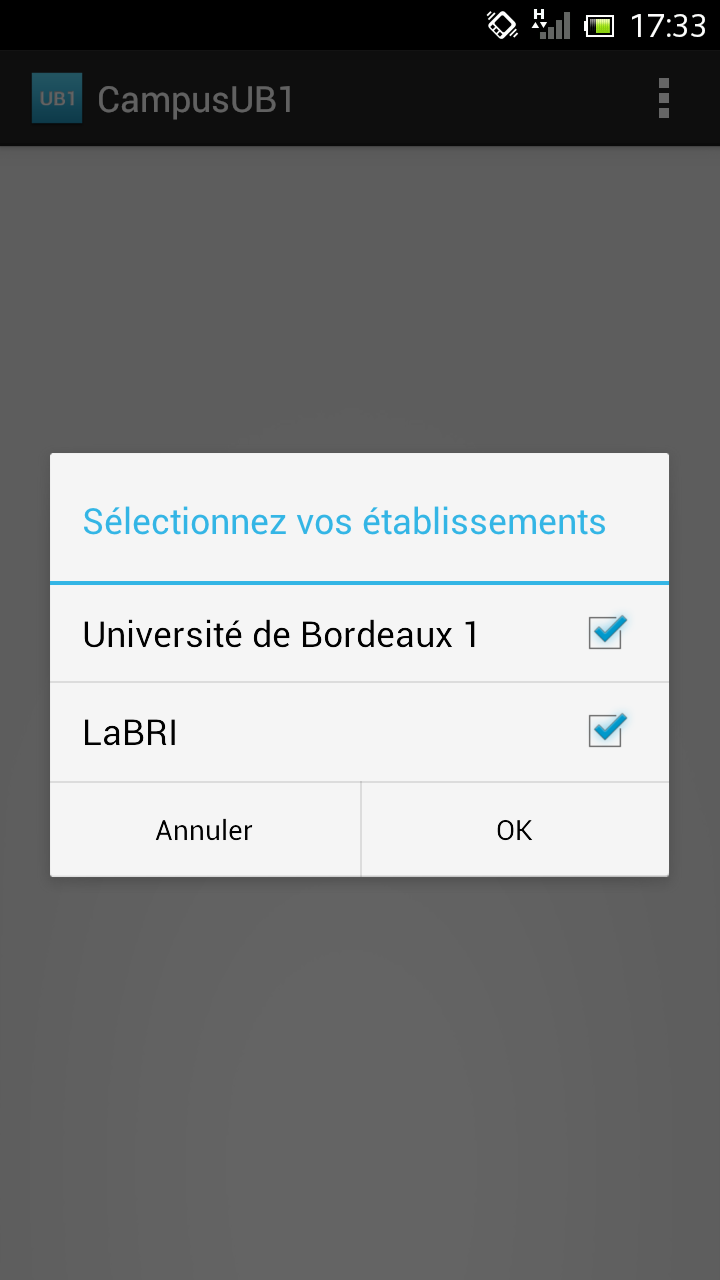
\includegraphics[width=0.8\textwidth]{resources/ui_preview/01}
    \caption{Lors du premier lancement de l'application, l'utilisateur doit sélectionner ses établissements. Une fois ses choix effectués, il sont enregistrés et ne seront plus demandés. Les établissements sont modifiables via les préférences.}
    \label{fig:01}
  \end{minipage}
  \hspace{+20pt}
  \begin{minipage}[t]{8cm}
    \centering
    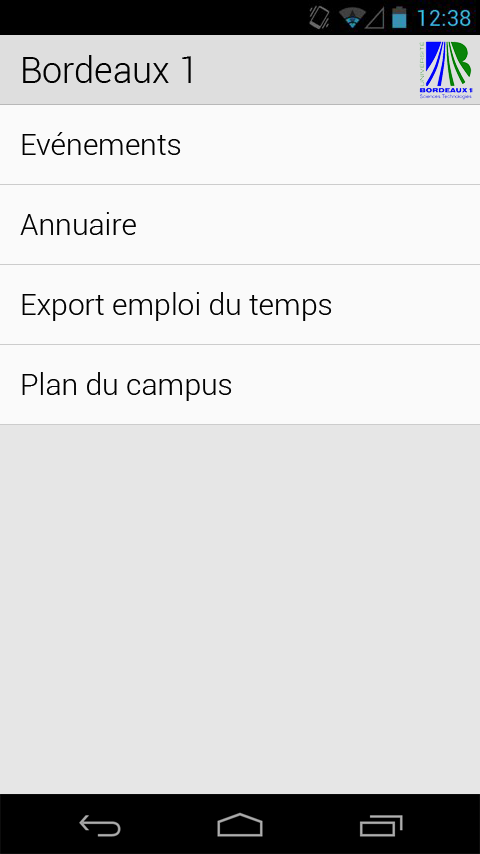
\includegraphics[width=0.8\textwidth]{resources/ui_preview/02}
    \caption{Vue d'accueil de l'application}
    \label{fig:02}
  \end{minipage}
  \hspace{-60pt}
\end{figure}


\begin{figure}
  \begin{minipage}[t]{8cm}
    \centering
    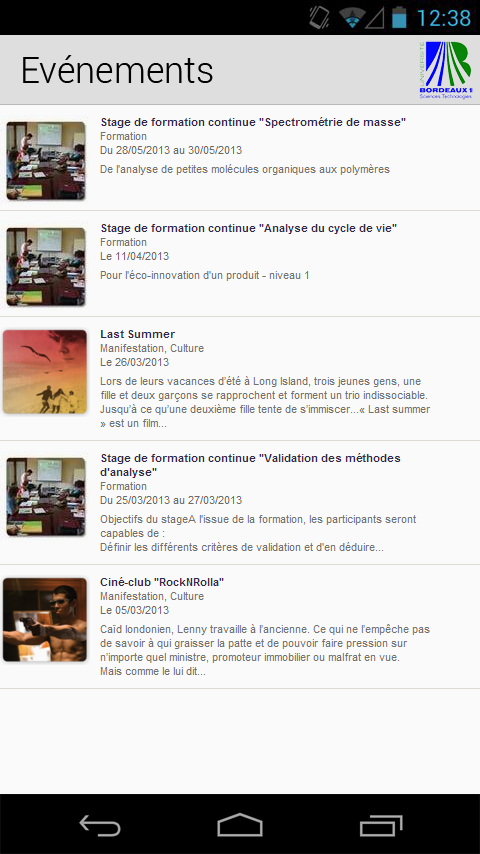
\includegraphics[width=0.8\textwidth]{resources/ui_preview/03}
    \caption{Vue des filtres des résultats en fonction des établissements préalablement choisis. Cette fonctionnalité est accessible en touchant le logo (situé en haut à gauche) de l'application uniquement depuis l'écran d'accueil.}
    \label{fig:03}
  \end{minipage}
  \hspace{+20pt}
  \begin{minipage}[t]{8cm}
    \centering
    
\includegraphics[width=0.8\textwidth]{resources/ui_preview/04}
    \caption{Vue des événements. Pour lire la news et arriver sur l'écran de la figure~\ref{fig:06}, il suffit de toucher la news correspondante. Par défaut, toutes les news sont affichées. On a également la possibilité de les afficher par catégories. La liste des catégories est disponible via la touche menu.}
    \label{fig:04}
  \end{minipage}
  \hspace{-60pt}
\end{figure}


\begin{figure}
  \begin{minipage}[t]{8cm}
    \centering
    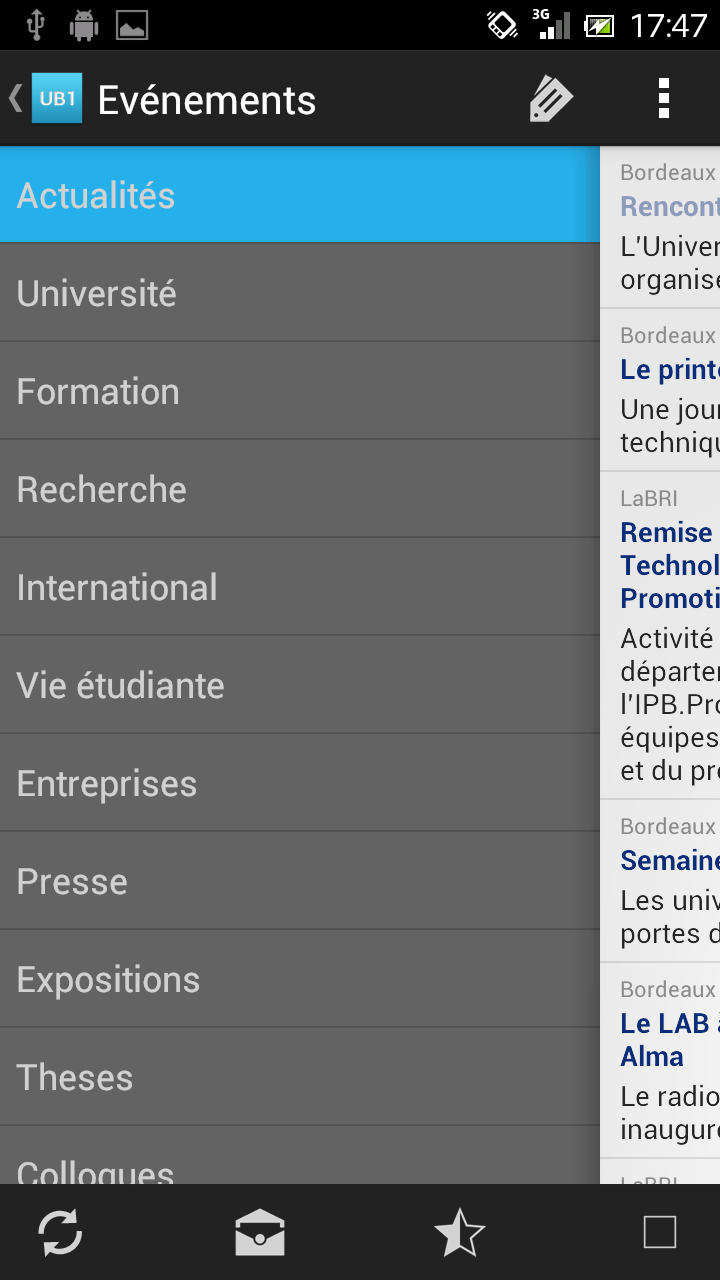
\includegraphics[width=0.8\textwidth]{resources/ui_preview/05}
    \caption{Liste des catégories pour afficher les news.}
    \label{fig:05}
  \end{minipage}
  \hspace{+20pt}
  \begin{minipage}[t]{8cm}
    \centering
    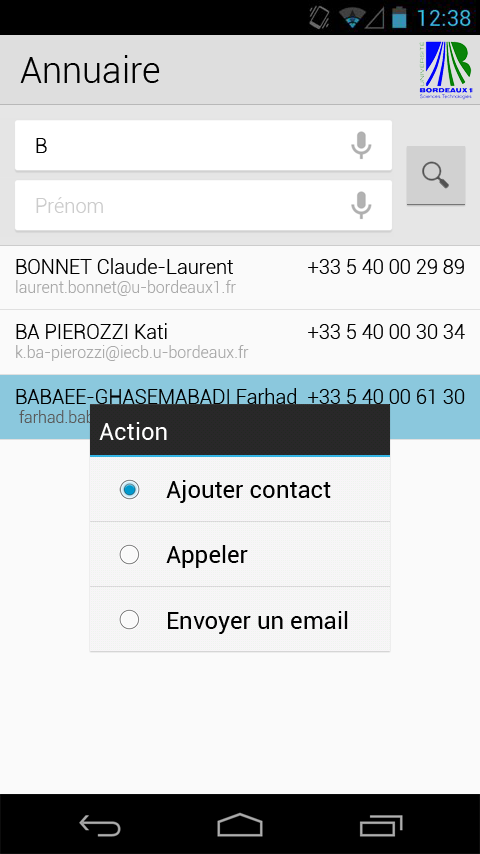
\includegraphics[width=0.8\textwidth]{resources/ui_preview/06}
    \caption{Vue détaillée d'une news. Le bouton ``plus'' situé en haut à droite permet d'ajouter l’événement au calendrier du smartphone.}
    \label{fig:06}
  \end{minipage}
  \hspace{-60pt}
\end{figure}


\begin{figure}
  \begin{minipage}[t]{8cm}
    \centering
    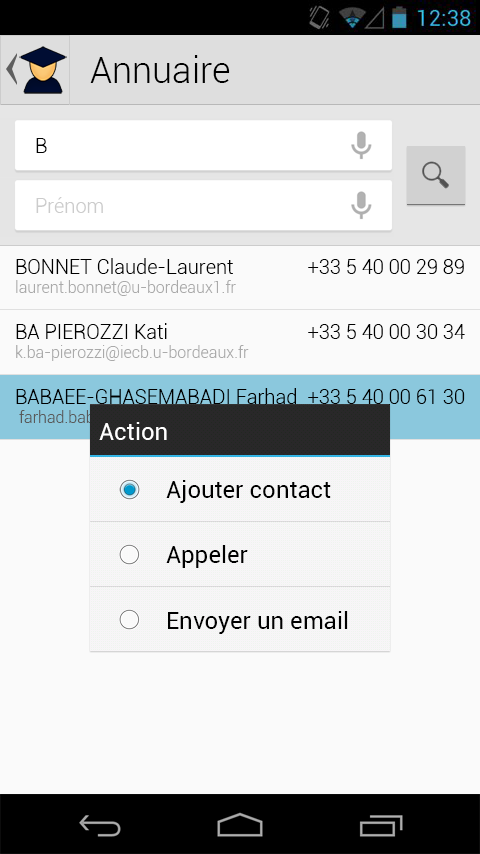
\includegraphics[width=0.8\textwidth]{resources/ui_preview/07}
    \caption{Vue de l'annuaire.}
    \label{fig:07}
  \end{minipage}
  \hspace{+20pt}
  \begin{minipage}[t]{8cm}
    \centering
    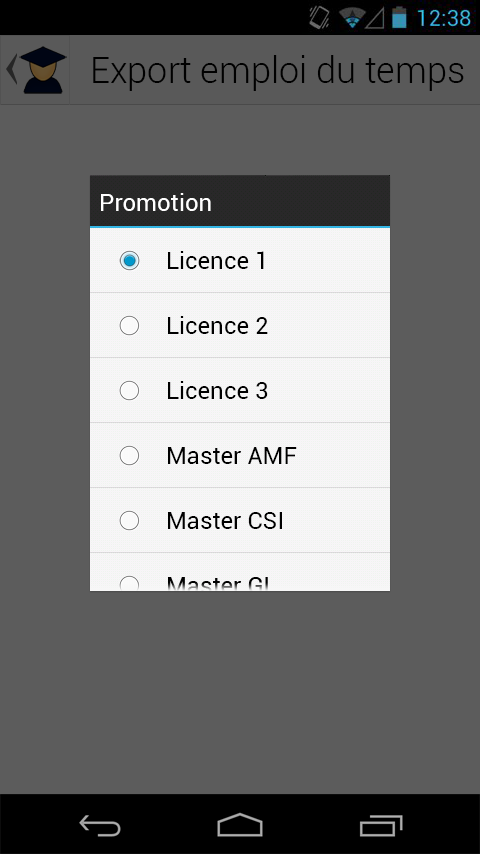
\includegraphics[width=0.8\textwidth]{resources/ui_preview/08}
    \caption{Vue des résultats de l'annuaire.}
    \label{fig:08}
  \end{minipage}
  \hspace{-60pt}
\end{figure}


\begin{figure}
  \begin{minipage}[t]{8cm}
    \centering
    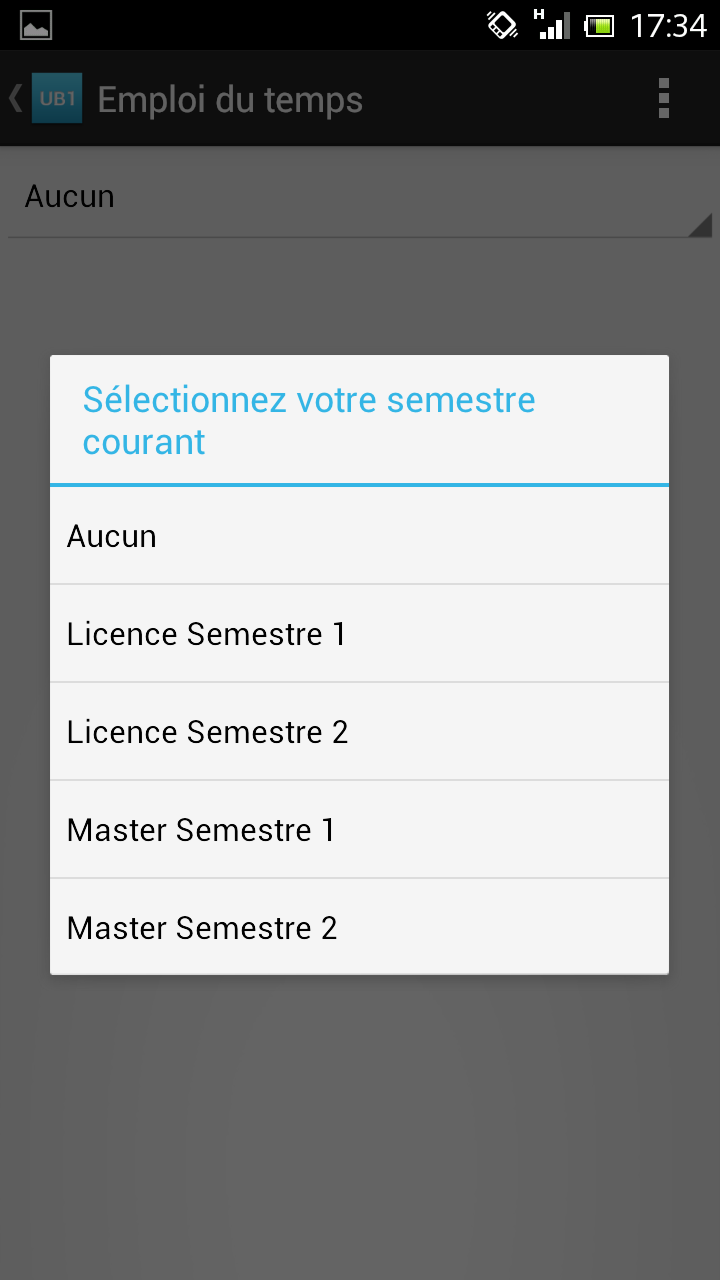
\includegraphics[width=0.8\textwidth]{resources/ui_preview/09}
    \caption{Export de l'emploi du temps. L'application demande la promotion seulement la première fois et il faudra aller dans les paramètres pour la modifier ultérieurement.}
    \label{fig:09}
  \end{minipage}
  \hspace{+20pt}
  \begin{minipage}[t]{8cm}
    \centering
    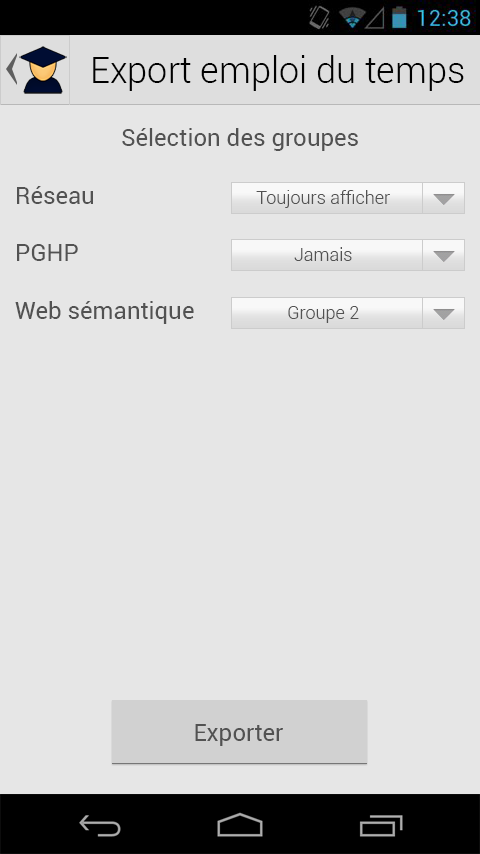
\includegraphics[width=0.8\textwidth]{resources/ui_preview/10}
    \caption{Sélection des groupes pour l'export de l'emploi du temps.}
    \label{fig:10}
  \end{minipage}
  \hspace{-60pt}
\end{figure}


\bibliography{biblio}
\end{document}
 
